% \setbeamerfont{alerted text}{series=\bfseries\large}
\setbeamertemplate{navigation symbols}{}
\usefonttheme[onlymath]{serif}

\setlength{\parskip}{1em}


\usepackage[utf8]{inputenc}
\usepackage[T1]{fontenc}
\usepackage{lmodern}
\usepackage{makecell} %...used in tabular for \thead
 
%...For highlighting
\usepackage{xcolor, soul} 
\makeatletter
\let\HL\hl
\renewcommand\hl{%
  \let\set@color\beamerorig@set@color
  \let\reset@color\beamerorig@reset@color
  \HL}
\makeatother

\hypersetup{
    colorlinks=true,
    linkcolor=blue,
    filecolor=magenta,      
    urlcolor=cyan,
    pdftitle={Overleaf Example},
    pdfpagemode=FullScreen,
}

\usepackage[acronym]{glossaries}
\glsdisablehyper %...disables hyperlinks for glossary terms in frames


\usepackage{amsmath}  %...for the equation* environment

%...Tikz and PGF packages
\usepackage{tikz}
\usetikzlibrary{calc,math}
\usetikzlibrary{patterns}
\usepackage{tikz-cd}
\usepackage{pgfplots}
\pgfplotsset{compat=1.18}
\usetikzlibrary{backgrounds} %...For shading portions of graphs
% \usetikzlibrary{math}
\tikzset{>=latex} %...For pretty arrows
\tikzset{
    declare function = {trajectoryequationTEN(\x,\vi,\thetai)= tan(\thetai)*\x - 10*\x^2/(2*(\vi*cos(\thetai))^2);},
    declare function = {trajectoryequation(\x,\vi,\thetai)= tan(\thetai)*\x - 9.8*\x^2/(2*(\vi*cos(\thetai))^2);},
    declare function = {patheq(\x,\yi,\vi,\thetai)= \yi + tan(\thetai)*\x - 9.8*\x^2/(2*(\vi*cos(\thetai))^2);}
} %...Plots the trajectory equation for projectile motion:


\usetikzlibrary{positioning}
\tikzset{onslide/.code args={<#1>#2}{%
  \only<#1>{\pgfkeysalso{#2}} % \pgfkeysalso doesn't change the path
}}

%...SI Units
\usepackage{siunitx}
%\sisetup{per-mode=fraction}
\usepackage{cancel}
\DeclareSIUnit{\mile}{mi}


%...Symbols packages
\usepackage{fontawesome} % for \faHome
\usepackage{tikzsymbols} % for tree and stick figure
\usepackage{twemojis} %...for twitter emojis
\usepackage{utfsym}  %...for a basic star symbol

%...Breaks long URLs
\usepackage{xurl}

%...Multiple columns for table of contents
\usepackage{multicol}

%...beamer specific
\AtBeginSection[]
{
  \begin{frame}
    \frametitle{Table of Contents}
    \begin{multicols}{2}
        \tableofcontents[currentsection]
    \end{multicols}
  \end{frame}
}

\setbeamerfont{frametitle}{size=\normalsize}

%...Vector commands
\newcommand{\bvec}[1]{\vec{\mathbf{#1}}}
\newcommand{\bhat}[1]{\,\hat{\mathbf{#1}}}


%%%%%%% DST, XVT, and VAT Triangles
\newcommand{\DSTtriangle}[1][]{%
    % Key-value setup for the shade argument
    \pgfkeys{/DST/.cd, shade/.store in=\DSTshade, shade=none, #1}%
    
    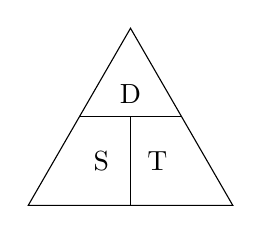
\begin{tikzpicture}[x=1.5cm,y=1.5cm]
        \coordinate (D) at (0,1);
        \coordinate (S) at ({cos(210)},{sin(210)});
        \coordinate (T) at ({cos(330)},{sin(330)});
        
        % Midpoints
        \coordinate (M1) at ($(D)!0.5!(S)$);
        \coordinate (M2) at ($(D)!0.5!(T)$);
        \coordinate (M3) at ($(M1)!0.5!(M2)$);
        \coordinate (M4) at ($(S)!0.5!(T)$);
        
        % Variables for comparison
        \def\shadeD{D}
        \def\shadeS{S}
        \def\shadeT{T}
        
        % Shading logic (drawn first so lines appear on top)
        \ifx\DSTshade\shadeD
            \fill[gray!30] (D) -- (M1) -- (M2) -- cycle;
        \fi
        \ifx\DSTshade\shadeS
            \fill[gray!30] (S) -- (M4) -- (M3) -- (M1) -- cycle;
        \fi
        \ifx\DSTshade\shadeT
            \fill[gray!30] (T) -- (M4) -- (M3) -- (M2) -- cycle;
        \fi
        
        % Triangle outer border
        \draw (D) -- (S) -- (T) -- cycle;
        
        % Lines between midpoints
        \draw (M1) -- (M2) node[pos=0.5,above=0.03] {D};
        \draw (M3) -- (M4) node[pos=0.5,left=0.1] {S} node[pos=0.5,right=0.06] {T};
    \end{tikzpicture}
}

\newcommand{\XVTtriangle}[1][]{%
    % Key-value setup for the shade argument
    \pgfkeys{/DST/.cd, shade/.store in=\DSTshade, shade=none, #1}%
    
    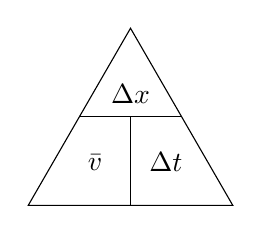
\begin{tikzpicture}[x=1.5cm,y=1.5cm]
        \coordinate (D) at (0,1);
        \coordinate (S) at ({cos(210)},{sin(210)});
        \coordinate (T) at ({cos(330)},{sin(330)});
        
        % Midpoints
        \coordinate (M1) at ($(D)!0.5!(S)$);
        \coordinate (M2) at ($(D)!0.5!(T)$);
        \coordinate (M3) at ($(M1)!0.5!(M2)$);
        \coordinate (M4) at ($(S)!0.5!(T)$);
        
        % Variables for comparison
        \def\shadeD{X}
        \def\shadeS{V}
        \def\shadeT{T}
        
        % Shading logic (drawn first so lines appear on top)
        \ifx\DSTshade\shadeD
            \fill[gray!30] (D) -- (M1) -- (M2) -- cycle;
        \fi
        \ifx\DSTshade\shadeS
            \fill[gray!30] (S) -- (M4) -- (M3) -- (M1) -- cycle;
        \fi
        \ifx\DSTshade\shadeT
            \fill[gray!30] (T) -- (M4) -- (M3) -- (M2) -- cycle;
        \fi
        
        % Triangle outer border
        \draw (D) -- (S) -- (T) -- cycle;
        
        % Lines between midpoints
        \draw (M1) -- (M2) node[pos=0.5,above=0.03] {$\Delta x$};
        \draw (M3) -- (M4) node[pos=0.5,shift={(-0.3,-0.01)}] {$\bar{v}$} node[pos=0.5,shift={(0.3,-0.01)}] {$\Delta t$};
    \end{tikzpicture}
}

\newcommand{\VATtriangle}[1][]{%
    % Key-value setup for the shade argument
    \pgfkeys{/DST/.cd, shade/.store in=\DSTshade, shade=none, #1}%
    
    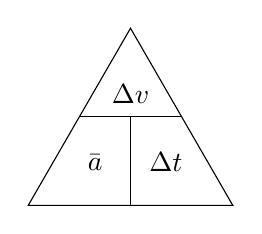
\begin{tikzpicture}[x=1.5cm,y=1.5cm]
        \coordinate (D) at (0,1);
        \coordinate (S) at ({cos(210)},{sin(210)});
        \coordinate (T) at ({cos(330)},{sin(330)});
        
        % Midpoints
        \coordinate (M1) at ($(D)!0.5!(S)$);
        \coordinate (M2) at ($(D)!0.5!(T)$);
        \coordinate (M3) at ($(M1)!0.5!(M2)$);
        \coordinate (M4) at ($(S)!0.5!(T)$);
        
        % Variables for comparison
        \def\shadeD{V}
        \def\shadeS{A}
        \def\shadeT{T}
        
        % Shading logic (drawn first so lines appear on top)
        \ifx\DSTshade\shadeD
            \fill[gray!30] (D) -- (M1) -- (M2) -- cycle;
        \fi
        \ifx\DSTshade\shadeS
            \fill[gray!30] (S) -- (M4) -- (M3) -- (M1) -- cycle;
        \fi
        \ifx\DSTshade\shadeT
            \fill[gray!30] (T) -- (M4) -- (M3) -- (M2) -- cycle;
        \fi
        
        % Triangle outer border
        \draw (D) -- (S) -- (T) -- cycle;
        
        % Lines between midpoints
        \draw (M1) -- (M2) node[pos=0.5,above=0.03] {$\Delta v$};
        \draw (M3) -- (M4) node[pos=0.5,shift={(-0.3,-0.01)}] {$\bar{a}$} node[pos=0.5,shift={(0.3,-0.01)}] {$\Delta t$};
    \end{tikzpicture}
}

%...Speedometer
\newcommand{\speedometer}[3]{%
    % #1: X-shift (y is fixed at 2) (e.g., 1)
    % #2: Needle rotation angle (e.g., 20)
    % #3: Top label (e.g., \texttt{Speed})
    % #4: Bottom readout (e.g., \textsf{32.0\,m/s})
    \begin{scope}[shift={#1},x=1.3cm,y=1.3cm]
        \draw (0,0) circle (1);
        \foreach \x in {340,360,...,560} {
            \coordinate (P) at ({cos(\x)},{sin(\x)});
            \draw[ultra thick,gray] (P) -- ($(P)!0.16!(0,0)$);
        }
        \foreach \x in {350,370,...,550} {
            \coordinate (P) at ({cos(\x)},{sin(\x)});
            \draw[thick,gray] (P) -- ($(P)!0.08!(0,0)$);
        }
        \fill (0,0) circle (0.02);
        \draw[fill=lightgray,rotate={#2},red] (0,0.02) rectangle (0.975,-0.02);
        \node at (0,0.4) {\texttt{Speed}};
        \draw[rounded corners] (-0.65,-0.75) rectangle ++(1.3,0.5) node[pos=0.5] {\textsf{#3\,m/s}};
    \end{scope}
}

